\documentclass[10pt]{article}\usepackage[margin=.65in]{geometry}\usepackage[T1]{fontenc}\usepackage{graphicx}\setlength{\parindent}{0pt}\setlength{\parskip}{7pt}\sloppy\begin{document}{\large Independent fast polynomial-call review}\par The non-author reviewer reports machine passed and faithful scoped correspondence for the five modeled polynomial-call/output declarations at aa3e94c0e6834aa1b5de2156c7c5128cabd64e23. Fresh replay, source review and exact input custody are archived separately from the producer packet.\par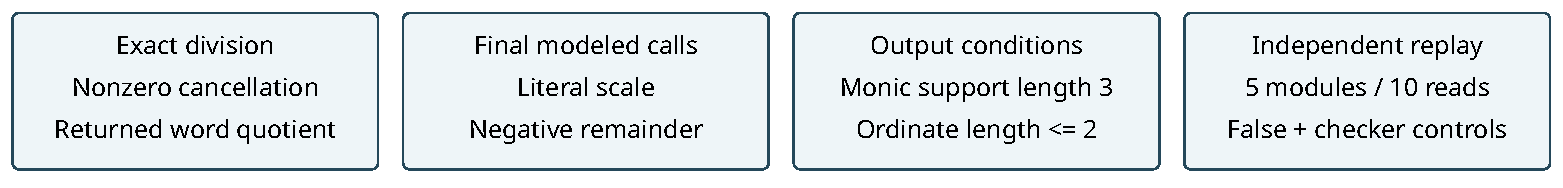
\includegraphics[width=\linewidth]{diagram.pdf}\par Checked construction. Input-list coefficient order and trimming match the intended native inputs. Proved nonzero input product permits cancellation that identifies the successful exactDiv word quotient with the field quotient. Literal computed inverse-leading scaling gives canonical normalized monic degree-two support. The final remainder is of negative V, with an explicit successful return equality. Support length exactly three and ordinate length at most two discharge the strict constructor length assertion.

Verification. Five modules, five fixed controls and ten exact named axiom readbacks passed. The deliberately false theorem was rejected with exit one, and three malformed checker inventories were rejected. Source, helper and compiler bindings remained unchanged. No unexpected replay failure occurred. Target module caches were freshly produced; deeper dependencies were reused and hash-bound rather than independently rebuilt or binary-rechecked.

Wording clarification. Operand nesting and value correspondence are established; global temporal scheduling is not modeled. Native code computes V before U, while the proof first names evidence for U. That ordering of proof evidence introduces no source-value mismatch and is not a temporal execution claim. The full F17 fixture constructs kernel-checked existential modeled outputs; it is not a separate numeric Rust execution.

Scope and next steps. The reviewed endpoint retains original canonical input words, prime modulus and explicit no-overflow bound, actual guards, degree-five curve polynomial and input residual divisibilities. Remaining joints are stored input extraction, full dispatch, final struct copy, fast/fallback equality and divisor-class interpretation. A later array-copy producer component is separate evidence and is not retroactively included in this review.

Independence and record. The reviewer authored none of the assigned modules, read no sibling new reports and inspected current main separately. Historical context was inherited, not blindly re-derived. Exact sources\_read, replay commands, logs, checker source, bindings and standard JSON outcome are retained. Original absolute paths require adaptation to a fresh private snapshot. Large binding files use the artifact store. No scientific status, cohort, timing, cost ratio or campaign limit changed.
\end{document}